\chapter{User Study}
\label{chp:b3}

\section{Dataset}

The set of images used in visual similarity experiments should be sufficiently diverse. Although such datasets exists for LDR images, there is no specific similarity dataset for HDR images. However, there exists HDR image datasets that were created for various purposes and by different authors. We therefore decided to select 100 HDR images from various such sources to present observers with a diverse set of images2. The used datasets were: Fairchild’s HDR Photographic Survey~\cite{fairchild2007hdr}, HDR-Eye~\cite{nemoto2015visual}, DEIMOS~\cite{klima2011deimos}, Empa HDR Image Database~\cite{EmpaHDR}, and pfstools HDR Image Gallery ~\cite{mantiuk2007high}. Thumbnails for the used images are shown in Figure \ref{fig:dataset}.

\begin{figure}
\begin{center}
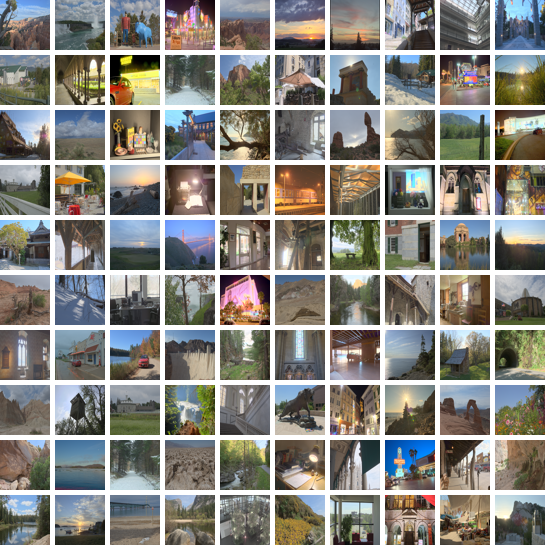
\includegraphics[width=\textwidth]{figures/chapter3/dataset.png}
\caption{HDR images used in the visual similarity experiments.}
\label{fig:dataset}
\end{center}
\end{figure}


\section{Experiment Setting}
%paper
To measure perceptual similarity between HDR images, we conducted a 2AFC experiment. The experiment is publicly available\footnote{http://user.ceng.metu.edu.tr/~merve/userstudy/}. As we needed a large number of responses, we designed a web-based interface to collect crowdsourcing data. We used the HDRHTML technique~\cite{mantiuk2009visualizing} for visualizing HDR images on web browsers.

This technique uses a windowing approach to select a desired exposure range from the HDR image. Multiple exposures are encoded by combining a small set of basis images with opacity coefficients. The tone-curves of these basis images are approximated as a piece-wise linear function. Instead of finding optimal tone-curves and opacity coefficients, HDRHTML uses a precomputed optimal solution and use these tone-curve points and opacity coefficients for all images for fast processing. After basis images are created using the tone-curves, these basis images are used to reconstruct multiple exposures and gives user the control over exposure settings with a slider. By dynamically adjusting the position of the slider, the user can efficiently view the entire exposure range contained within the HDR image. These sliders are normally overlayed with the image histogram. We removed this overlay to prevent the image histogram from affecting the observers’ decisions. Figure \ref{fig:experiment} shows a sample trial from the experiment. An HDR reference image was shown at the top and two HDR test images were shown at the bottom. The sliders, which were mandatory to be adjusted, allowed all images to be inspected at different exposure levels.

\begin{figure}
\begin{center}
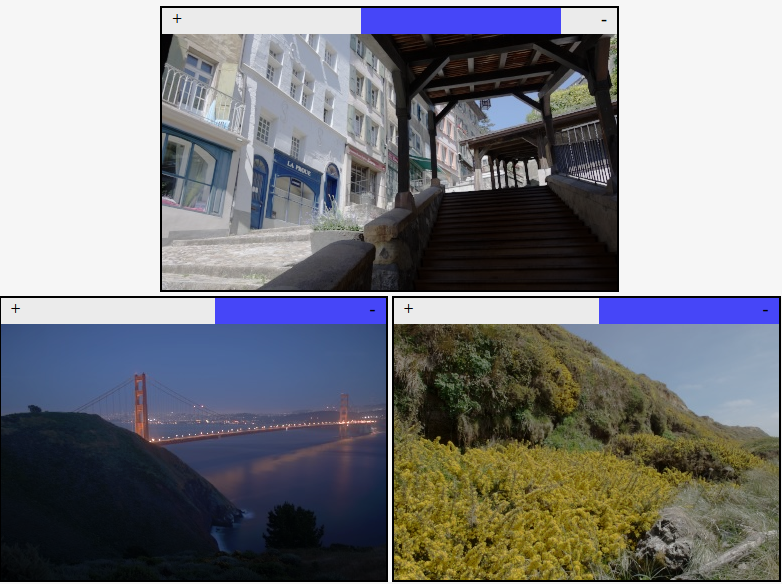
\includegraphics[width=\textwidth]{figures/chapter3/experiment.png}
\caption{EA sample trial from the experiment. The observers were asked to choose the most similar image to the reference image (top) from the test images (bottom). All images could be examined at different exposure levels by adjusting their sliders.
%paper
}
\label{fig:experiment}
\end{center}
\end{figure}

In each experimental session, 33 such image triplets were displayed to the observers. Thus, an experimental session consisted of 33 trials. In each trial, the observers were asked to choose which of the two test images was visually more similar to the reference image. Here it is important to note that we did not ask users to decide for a specific type of similarity such as object, color, etc. By intentionally leaving the definition of visual similarity vague, we hoped to achieve a range of responses, which in overall, would converge to a common sense understanding for similarity. All trials, except for the verification ones, were generated randomly from the dataset during the runtime of the experiment. 

Three of the experiment triplets were used for verification. They contained an obviously similar reference and test image pair to evaluate the reliability of an observer as shown in Figure \ref{fig:verficiation}. As seen from the figure, the test image that is similar to the reference image is another image from the same scene. These images are not used in the actual part of the experiment, and do not belong to the dataset of 100 images shown in Figure \ref{fig:dataset}.

\begin{figure}
\begin{center}
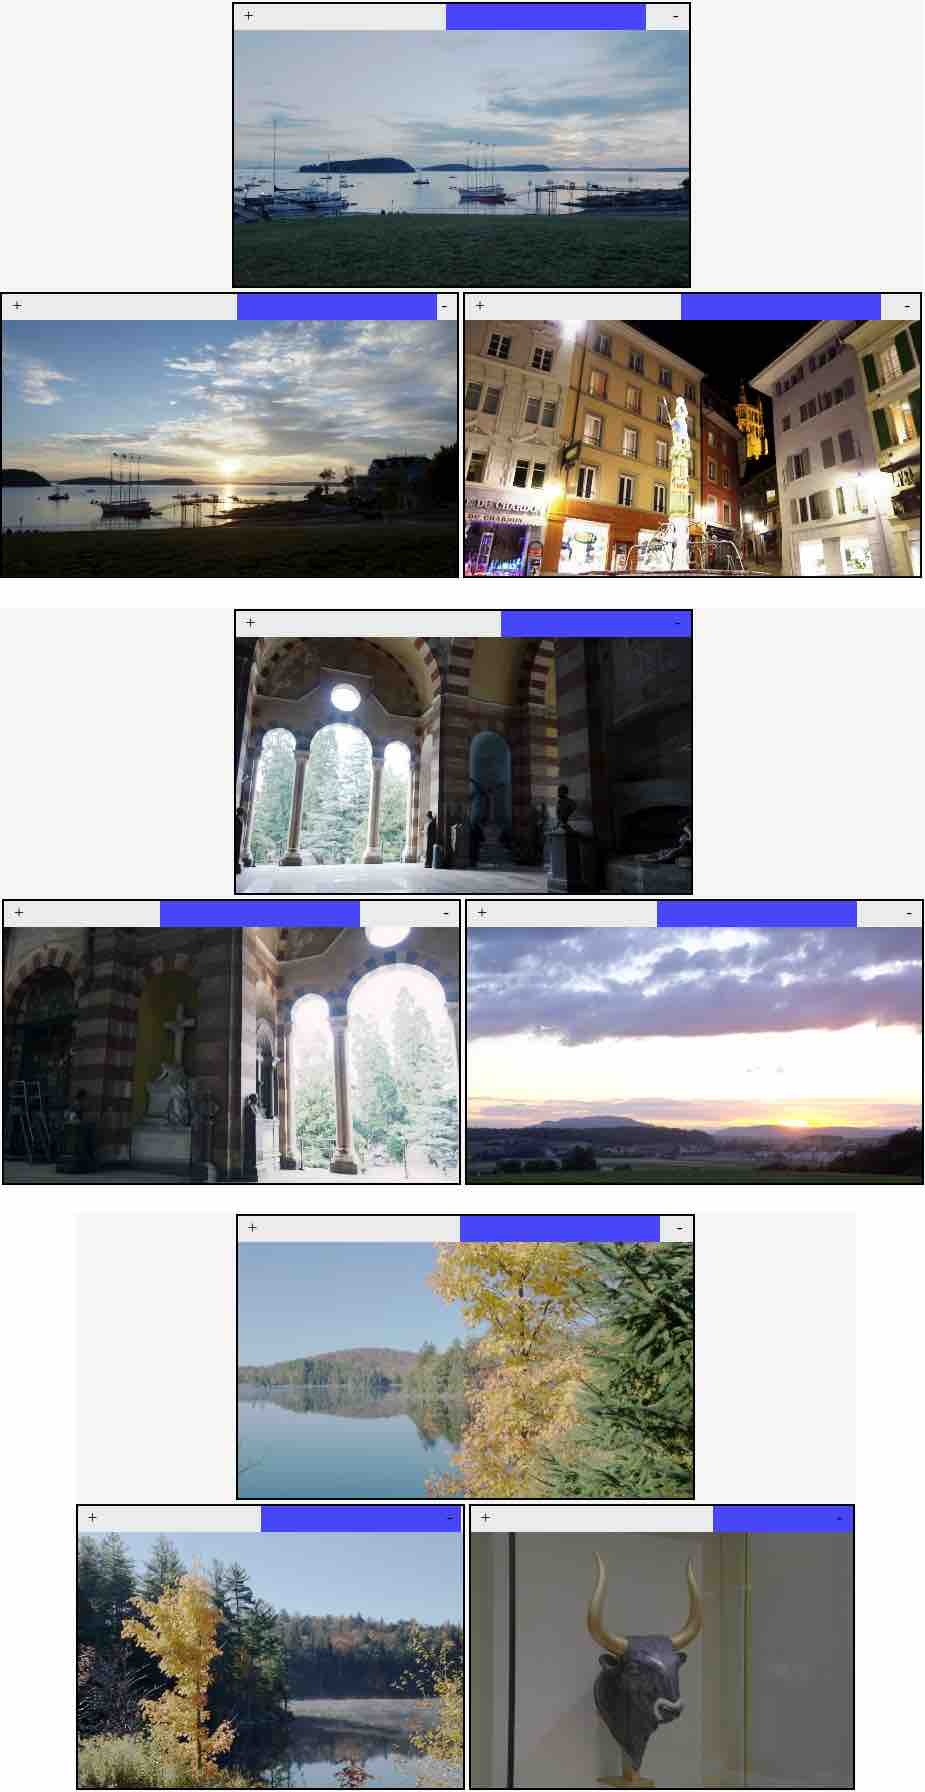
\includegraphics[height=0.85\textheight]{figures/chapter3/verification_small.jpg}
\caption{Verification triplets, shown as 3rd, 10th and 16th trials in the experiment sessions. }
\label{fig:verficiation}
\end{center}
\end{figure}

If an observer failed to provide the correct answer even for one of these trials, his or her data was discarded as being unreliable. These trials were distributed across the experiment to ensure that observers were attentive throughout. Before the experiment began, observers were informed about their task and the expected duration of the experiment, which was at most 20 minutes at a normal pace. During the experiment, observers were required to use the exposure sliders for each image before they made selection. Image selection was done by clicking on one of the test images. The selection was indicated using a green border around the selected image. Observers could change their selection until they pressed the “Next” button. The progress of an observer was indicated using a small progress bar at the bottom center of the screen. At the end of the experiment, observers were informed with a final page confirming the conclusion of the experiment and were presented with unique session ids. They were required to enter this id to the crowdsourcing platform to verify that they have finished the experiment.

\section{Data Collection}
Crowdsourcing has been used in many computer vision problems to collect non-expert data~\cite{kovashka2016crowdsourcing}. In this thesis, in order to reach as many people as possible, the experiment was published at Microworkers crowdsourcing platform\footnote{www.microworkers.com}. For each completed experiment 0.3\$ were paid to the participants.

One of the challenges of data crowdsourcing is eliminating users that give unreliable responses, this may due to not being qualified for the task or just being a spammer~\cite{garcia2016challenges}. To minimize the problem of users being not qualified, the crowd group of English speaking, high qualified users are selected from the crowdsourcing platform. Even though the experiment itself does not require language proficiency, the instructions at the beginning of the experiment is important for users to successfully complete the experiment. The users are in the \emph{high qualified} crowd, if they have been done other crowdsourcing tasks before and got positive feedback. Another measure taken to achieve reliable responses is using verification triplets.

In total, 165 sessions were discarded due to incorrect responses given to the verification trials. Age, gender, and familiarity with computer graphics/image processing distribution of the participants are shown in Figure \ref{fig:age_gender_cgi}. This information was asked to the users at the beginning of the experiment.

\begin{figure}
\begin{center}
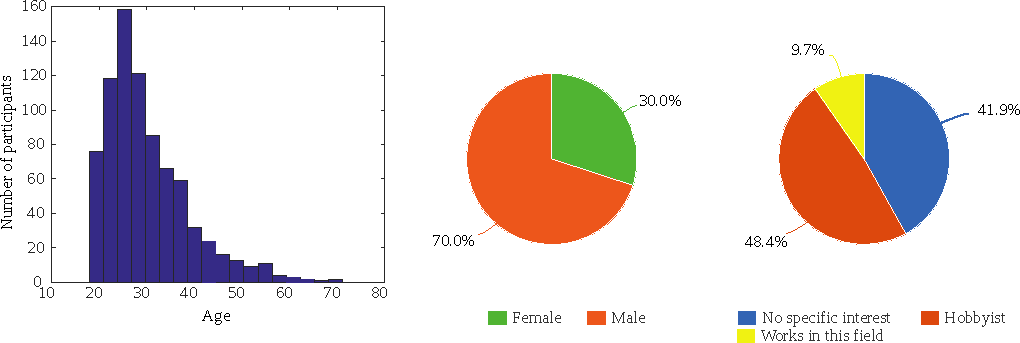
\includegraphics[width=\textwidth]{figures/chapter3/age_gender_cgi.pdf}
\caption{Age, gender, and computer graphics/image processing familiarity distribution of the participants.
%paper
}
\label{fig:age_gender_cgi}
\end{center}
\end{figure}

\subsection{Phase I}
\label{sec:exp_phase_I}
In the first phase of the experiment, randomly selected triplets are shown to the users without any restrictions on the image selection. After collecting the experimental results, and eliminating the triplets from invalid sessions, it was found that 18747 unique image triplets were judged by the observers. This amounts to approximately 11.6\% of the total possible triplets that can be obtained from 100 images, $C(100, 3)$. Experiment sessions were independent and random for each participant, but it was guaranteed that a single session consisted of only unique triplets. 

This design resulted in a single response for the majority of the triplets. Some triplets received two responses and only a few received three or more. As such this first phase of the experiment is considered as a random exploration of all possible comparisons. However, as judging similarity based on a single response could be too subjective, the experiment is extended as discussed below to collect multiple responses for each triplet.

\subsection{Phase II}
\label{sec:exp_phase_II}
The first phase of the experiment was extended to obtain three evaluations per triplet. Unlike the first phase where triplets were generated randomly, the second phase solely used the triplets that had been evaluated in the first phase of the experiment. To achieve this, the triplets sorted from the first phase in descending order by the number of responses collected. If a triplet had more than three responses, three of the responses are randomly selected. The triplets with exactly three responses were used as is. These two cases occurred very rarely. Next, triplets with two responses, and then a single response were presented randomly to obtain a total of 4990 triplets that had been evaluated three times. Among these thrice evaluated triplets, 2170 triplet were judged consistently by all three observers. The remaining 2820 triplets generated two-to-one responses. Similar to the first part of the experiment, the second part also contained the same validity checks to eliminate the responses of inattentive observers.










